\begin{figure}[h!]
	\centering
	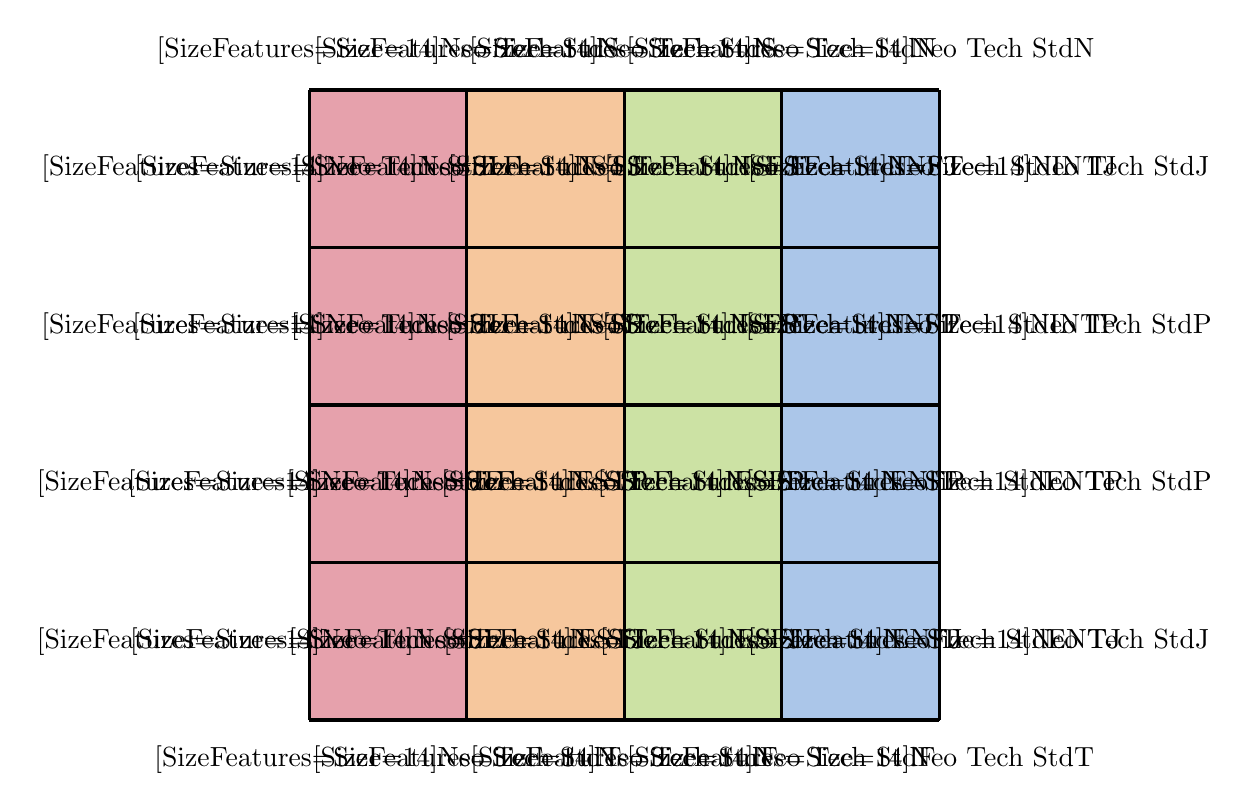
\begin{tikzpicture}
		%\draw[thin, draw=LightSkyBlue, anchor=south west, step=1mm] (0,0) grid (10,10);
		%\draw[draw=blue,anchor=south west, step=5mm] (0,0) grid (10,10);
		%\draw[thick,draw=SkyBlue,anchor=south west, step=10mm] (0,0) grid (10,10);
		%
		%% DEFINE COLORS
		\definecolor{r1}{cmyk}{0.08,0.36,0.21,0}
		\definecolor{y1}{cmyk}{0.02,0.21,0.33,0}
		\definecolor{g1}{cmyk}{0.2,0.04,0.36,0}
		\definecolor{b1}{cmyk}{0.33,0.14,0.01,0}
		
		%% DEFINE COLORED REGIONS
		\draw[very thin, fill=r1] (1,1) -- (3,1) -- (3,9) -- (1,9) -- cycle;
		\draw[very thin, fill=y1] (3,1) -- (5,1) -- (5,9) -- (3,9) -- cycle;
		\draw[very thin, fill=g1] (5,1) -- (7,1) -- (7,9) -- (5,9) -- cycle;
		\draw[very thin, fill=b1] (7,1) -- (9,1) -- (9,9) -- (7,9) -- cycle;
		
		%% DRAW THE VERTICAL GRID
		\draw[very thick, black] (1,9) -- (9,9);
		\draw[very thick, black] (1,7) -- (9,7);
		\draw[very thick, black] (1,5) -- (9,5);
		\draw[very thick, black] (1,3) -- (9,3);
		\draw[very thick, black] (1,1) -- (9,1);
		
		%% DRAW THE HORIZONTAL GRID
		\draw[very thick, black] (9,1) -- (9,9);
		\draw[very thick, black] (7,1) -- (7,9);
		\draw[very thick, black] (5,1) -- (5,9);
		\draw[very thick, black] (3,1) -- (3,9);
		\draw[very thick, black] (1,1) -- (1,9);
		
		%% TOP LETTERS
		\node[black] at (2,9.5) {\fontspec[SizeFeatures={{Size=14}}]{Neo Tech Std}S};
		\node[black] at (4,9.5) {\fontspec[SizeFeatures={{Size=14}}]{Neo Tech Std}S};
		\node[black] at (6,9.5) {\fontspec[SizeFeatures={{Size=14}}]{Neo Tech Std}N};
		\node[black] at (8,9.5) {\fontspec[SizeFeatures={{Size=14}}]{Neo Tech Std}N};
		
		
		%% LEFT SIDE LETTERS
		\node[black] at (0.5,8) {\fontspec[SizeFeatures={{Size=14}}]{Neo Tech Std}I};
		\node[black] at (0.5,6) {\fontspec[SizeFeatures={{Size=14}}]{Neo Tech Std}I};
		\node[black] at (0.5,4) {\fontspec[SizeFeatures={{Size=14}}]{Neo Tech Std}E};
		\node[black] at (0.5,2) {\fontspec[SizeFeatures={{Size=14}}]{Neo Tech Std}E};
		
		%% RIGHT SIDE LETTERS
		\node[black] at (9.5,8) {\fontspec[SizeFeatures={{Size=14}}]{Neo Tech Std}J};
		\node[black] at (9.5,6) {\fontspec[SizeFeatures={{Size=14}}]{Neo Tech Std}P};
		\node[black] at (9.5,4) {\fontspec[SizeFeatures={{Size=14}}]{Neo Tech Std}P};
		\node[black] at (9.5,2) {\fontspec[SizeFeatures={{Size=14}}]{Neo Tech Std}J};
		
		%% BOTTOM LETTERS
		\node[black] at (2,.5) {\fontspec[SizeFeatures={{Size=14}}]{Neo Tech Std}T};
		\node[black] at (4,.5) {\fontspec[SizeFeatures={{Size=14}}]{Neo Tech Std}F};
		\node[black] at (6,.5) {\fontspec[SizeFeatures={{Size=14}}]{Neo Tech Std}F};
		\node[black] at (8,.5) {\fontspec[SizeFeatures={{Size=14}}]{Neo Tech Std}T};
		
		%% TYPE INDICATORS
		\node[black] at (2,8) {\fontspec[SizeFeatures={{Size=14}}]{Neo Tech Std}ISTJ};
		\node[black] at (2,6) {\fontspec[SizeFeatures={{Size=14}}]{Neo Tech Std}ISTP};
		\node[black] at (2,4) {\fontspec[SizeFeatures={{Size=14}}]{Neo Tech Std}ESTP};
		\node[black] at (2,2) {\fontspec[SizeFeatures={{Size=14}}]{Neo Tech Std}ESTJ};
		
		\node[black] at (4,8) {\fontspec[SizeFeatures={{Size=14}}]{Neo Tech Std}ISFJ};
		\node[black] at (4,6) {\fontspec[SizeFeatures={{Size=14}}]{Neo Tech Std}ISFP};
		\node[black] at (4,4) {\fontspec[SizeFeatures={{Size=14}}]{Neo Tech Std}ESFP};
		\node[black] at (4,2) {\fontspec[SizeFeatures={{Size=14}}]{Neo Tech Std}ESFJ};
		
		\node[black] at (6,8) {\fontspec[SizeFeatures={{Size=14}}]{Neo Tech Std}INFJ};
		\node[black] at (6,6) {\fontspec[SizeFeatures={{Size=14}}]{Neo Tech Std}INFP};
		\node[black] at (6,4) {\fontspec[SizeFeatures={{Size=14}}]{Neo Tech Std}ENFP};
		\node[black] at (6,2) {\fontspec[SizeFeatures={{Size=14}}]{Neo Tech Std}ENFJ};
		
		\node[black] at (8,8) {\fontspec[SizeFeatures={{Size=14}}]{Neo Tech Std}INTJ};
		\node[black] at (8,6) {\fontspec[SizeFeatures={{Size=14}}]{Neo Tech Std}INTP};
		\node[black] at (8,4) {\fontspec[SizeFeatures={{Size=14}}]{Neo Tech Std}ENTP};
		\node[black] at (8,2) {\fontspec[SizeFeatures={{Size=14}}]{Neo Tech Std}ENTJ};
	\end{tikzpicture}
	\caption[Jungs Type Indicator]{Skematisk opstilling af de 16 mulige personligheder som tillades jf. Jungs teori, \citep{jung1923psychological,JTI, Ringstad:2002, MBTI}.}
	\label{fig:MBTI}
\end{figure}